\section{Introdução}\label{sec:gen}

% - Qual é a da coisa? (sintese c webaudio)
% - como a coisa funciona? 
%   - como um ou outro fez funcionar
%   - nosso jeito de funcionar

% -----------------------------------------------
 % http://www.charlie-roberts.com/pubs/Gibber_charles_roberts_icmc_2012.pdf


A \emph{Web Audio API} \cite{w3c_web_2012} possibilitou a emancipação de áudio generativo para jogos e aplicativos de síntese sonora em navegadores de rede tornando o navegador uma plataforma musical viável de diversas formas \cite{roberts_web_2013,wyse_viability_2014}.

% 
Esta API traz diversos \emph{nós de áudio} padrões que podem ser concatenados em um grafo de DSP.
Um exemplo desta concatenação pode ser vista na Figura \ref{fig:shime} onde são utilizados três nós diferentes em um sintetizador, em sequência: uma instância de oscilador de ondas (OscilatorNode), uma instância de ganho (GainNode) e uma última instância que representa os alto-falantes (DestinationNode).

\begin{figure}[h]
\centering
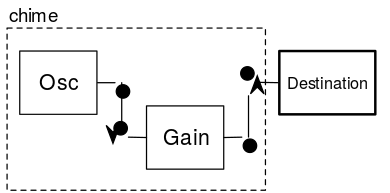
\includegraphics[scale=0.35]{chime.png}
\caption{Estrutura de síntese da API webaudio. \textbf{Fonte}: \cite{srikumar_tamming_2013}.}
\label{fig:shime}
\end{figure}

Um sintetizador mais complexo pode ter diversos nós concatenados, entre eles um nó ``especial'' chamado \emph{ScriptProcessorNode}, que permite o cálculo de cada \emph{sample} durante o processamento de sua saída.

Baseado nesta API e principalmente neste nó, alguns \emph{frameworks} são eles mesmos os instrumentos musicais; seja pelo encapsulamento de funcionalidades, seja pela maneira de pensar como o músico -- profissional ou amador -- codificará o processamento de sinais de áudio no navegador.
Entre estes \emph{frameworks}, destacam-se o trabalhos como \emph{Gibber} e \emph{Wavepot}. 

Este trabalho apresenta uma outra ferramenta \emph{open source}, desenvolvida a partir do estudo dos \emph{softwares} acima.
Chamamos de Termpot: \emph{Term} por uma questão de similaridade com um terminal de computador, inspirado no GROOVE de Max Mathews e \emph{Pot} por uma questão de similaridade técnica com o \emph{Wavepot}.
Nossa motivação foi desenvolver um \emph{framework} como uma plataforma de luteria composicional\cite{soares_luteria_2015} aberta e colaborativa, a partir de algumas reflexões de notação e execução musical.


A Seção \ref{sec:trabalhos} deste artigo apresenta os frameworks supracitados e uma breve comparação entre eles.
A Seção \ref{sec:termpot} apresenta a ferramenta proposta.
A Seção \ref{sec:resultados} traz os resultados desta pesquisa e a Seção \ref{sec:conclusao} apresenta as conclusões do trabalho até o presente momento.

